\section{SNLI as a platform for NLI research}

Since our goal is to evaluate the quality of the single sentence representations in our model, we train an entailment classifier that has access only to the output of our sentence representation model, and not to any of the word or phrase representations that it used. We encourage future users of this corpus to evaluate their models in this way when possible. Our classifier is simply a stack of three 100d (NONLIN) layers, with the bottom layer taking the concatenated sentence representations as input and the top layer feeding a softmax classifier, all trained jointly with the representation model itself.

\subsection{Baselines}

\subsection{Existing NLI systems}

\subsection{Sentence embeddings and NLI}\label{sentence-embedding}

\begin{figure}[tp]
  \centering
\scalebox{0.85}{
 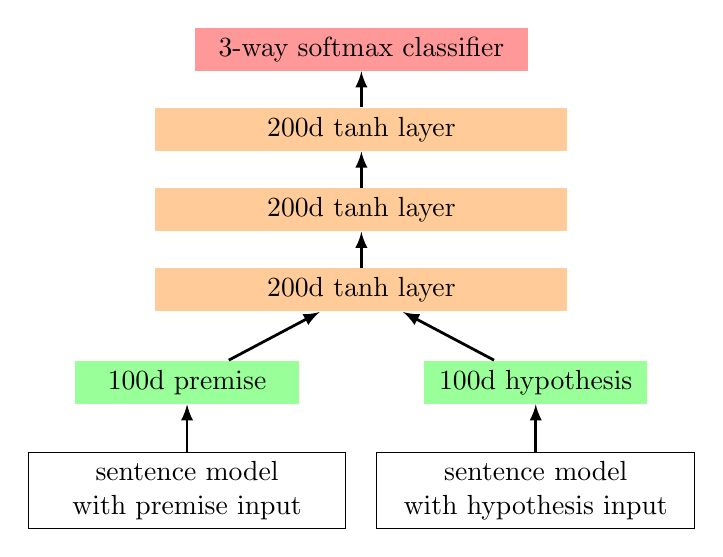
\begin{tikzpicture}
    \def\dx{21pt}
    \def\dy{29pt}

    \tikzstyle{label}=[text width=40mm,align=center]    
    \tikzstyle{softmax}=[fill=red!40,text width=40mm,align=center]
    \tikzstyle{preclass}=[fill=orange!40,text width=50mm,align=center]
    \tikzstyle{e}=[fill=green!40,text width=26mm,align=center]
    \tikzstyle{m}=[draw=black,text width=38mm,align=center]    
    
    \node[softmax]  (softmax) at (0*\dx,6*\dy) {3-way softmax classifier};
    \node[preclass]  (pc3) at (0*\dx,5*\dy) {200d $\tanh$ layer};
    \node[preclass]  (pc2) at (0*\dx,4*\dy) {200d $\tanh$ layer};
    \node[preclass]  (pc1) at (0*\dx,3*\dy) {200d $\tanh$ layer};
    \node[e]  (pe) at (-3*\dx,1.85*\dy) {100d premise};
    \node[e]  (he) at (3*\dx,1.85*\dy) {100d hypothesis};
    \node[m]  (pem) at (-3*\dx,0.5*\dy) {sentence model\\ with premise input};
    \node[m]  (hem) at (3*\dx,0.5*\dy) {sentence model\\ with hypothesis input};    
    
    \pgfsetarrowsend{latex}
    \tikzstyle{fwd} = [draw=black, line width=1pt]

          \draw [fwd] (pc3) -- (softmax);
          \draw [fwd] (pc2) -- (pc3);
          \draw [fwd] (pc1) -- (pc2);
          \draw [fwd] (pe) -- (pc1);
          \draw [fwd] (he) -- (pc1);
          \draw [fwd] (hem) -- (he);
          \draw [fwd] (pem) -- (pe);

  \end{tikzpicture}}
	
        \caption{The neural network classification architecture: for each sentence embedding model evaluated in \reftabs{tab:nnresults}{tab:transferresults}, two identical copies of the model are run with the two sentences as input, and their outputs are used as the two 100d inputs shown here.}
  \label{modelstructure}
\end{figure}


\subsection{Results}
